\documentclass[10pt]{article}
\usepackage{verbatim}
\usepackage{multirow}
\usepackage{fullpage}
\usepackage{graphicx}
\usepackage{parskip}
\usepackage{url}

\pagestyle{plain}

\title{{\normalsize CSCI 572: Computer Networks (Fall 2023)}\\Final Project: Ad-Hoc Messaging App}
\author{Michael Alvarez, Luke Beukelman, Ben Breisch}
\date{December 8th 2023}

\begin{document}

\maketitle

\section{Introduction}

If someone wants to send a message to a friend nearby, the message must travel much farther than the distance between devices. Messages sent through SMS or Apple's iMessage must travel from the originating device through a series of intermediate infrastructure nodes before reaching the destination device. This causes increased latency and unnecessary network overhead.

In an increasingly connected (and congested) world - why bother wasting bandwidth on a message to a nearby device that can be sent directly from peer to peer? We aim to solve this issue by proposing and developing a peer-to-peer messaging app for Android using Wi-Fi Direct. An application of this nature has far-reaching applications from messaging and networking at an event or conference, to emergency communication during a natural disaster where infrastructure may be lacking or damaged. 

\section{Requirements}

\begin{center}
    \begin{tabular}{| p{0.2\textwidth} | p{0.2\textwidth} | p{0.4\textwidth} |}
        \hline
        Category        & Name          & Description
        \\ \hline
        Networking      & WiFI Direct   & Connections between two devices shall use Wi-Fi Direct using the Android Wi-Fi P2P API
        \\ \hline
        Networking      & Ack           & Devices shall provide acknowledgements when messages are received in order to ensure message delivery
        \\ \hline
        User Experience & Contents      & Users shall be able to send text and file message
        \\ \hline
        User Experience & Latency       & Latency shall be minimized as much as possible when sending messages (ideally within 1 second)
        \\ \hline
        User Experience & Storage       & Devices shall save messages offline such that they can be viewed later
        \\ \hline
        User Experience & Neighbor List & Devices shall show a contact list of other nearby users that a user can start a conversation with
        \\ \hline
    \end{tabular}
\end{center}

\newpage

\section{Related work}

\subsection{Implementations}

\subsubsection{AirDrop}

When it comes to ad hoc networking on mobile devices, AirDrop is probably the most widespread application. It supports sending files to nearby devices, without requiring devices to be connected to the same network. AirDrop operates using both Wi-Fi and Bluetooth \cite{AppleSupport}.

We differ from this product in several regards:

\begin{enumerate}
    \item We primarily support messaging. Having file sharing as a back end is a possible implementation to build messaging on, but would need to be extended.
    \item AirDrop uses iCloud services in order to authenticate users \cite{AppleSupportSecurity}, and additionally only works on Apple devices. We aim to create a de-centralized version that could theoretically be deployed on any platform (although we are only developing the application for Android in the scope of this project).
    \item AirDrop uses a combination of point-to-point WiFi connections and bluetooth. We aim to use Wi-Fi Direct in our implementation. We realize that the technology choice restricts what devices we can connect with (mainly just in that Apple does not support Wi-Fi direct).
\end{enumerate}

\subsubsection{Warpinator}

Warpinator is a file sharing system devloped by the Linux Mint team in order to create an AirDrop like file-sharing system for non-Apple users  \cite{Webster2023linuxmint}. It operates over LAN, and supports Android, iOS, Windows, and Linux, and could likely be easily ported to other Unix like systems.

We differ from this product in two regards:

\begin{enumerate}
    \item Warpinator is similar to AirDrop in that it is primarily for file transfer, we primarily aim to support messaging.
    \item Operate using ad-hoc networking to support messaging. Warpinator requires a connection to an existing routed network, and can not operate its own ad-hoc network.
\end{enumerate}

\subsubsection{Android Beam}

Android beam is a discontinued \cite{Cantisano_2022} feature in Android that allowed data to be transfered over NFC \cite{AndroidDevelopers}. Unlike the prior two works, Android Beam did not only support file transfer, and was an open interface that applications could use to communicate. Android Beam could provide a reasonable interface for a similar application as ours to communicate with, if it were not discontinued and limited to NFC.

We differ from this product in two regards:

\begin{enumerate}
    \item We use WiFi technologies, rather than NFC, due to the short range limitation of NFC.
    \item We are creating an application, rather than an open interface to communicate over.
\end{enumerate}

\newpage

\subsection{Bridgefy}

Bridgefy is a messaging app that utilizes bluetooth that is available on Android and IOS \cite{Bridgefy}. It uses mesh networking, so messages can hop over multiple other devices supporting Bridgefy to get the the recipient. Bridgefy also supports end-to-end encryption.

We differ from this product in multiple regards:

\begin{enumerate}
    \item Bridgefy operates over Bluetooth. We prefer WiFi direct for its potentially longer range, as we do not anticipate that there will be substantial adoption to enable the advantages of mesh networking.
    \item Bridgefy has encryption and mesh networking considerations, which places it outside the scope of this project.
\end{enumerate}

\subsection{Papers}

\subsubsection{A Totally Decentralized Document Sharing System for Mobile Ad Hoc Networks}

This paper  \cite{10.1145/1164783.1164805} presents an application for sharing documents in MANETS. The application presented is completely unreliant on any form of centralized server or routing algorithms. Documents can be shared in atomic components to different groups of nodes, and nodes can modify parts of a document, sharing a tree of the modifications. This application achieves a lot of what we are trying to do, except with more routing and versioning complexity than we are seeking. Our goal is simple messaging and possible document sharing with nearby nodes, not necessarily using MANET routing algorithms.

We differ from this product in two regards:
\begin{enumerate}
    \item Our solution aims to target simple messaging and file sharing, rather than the complex sharing and versioning that the application in the paper presents.
    \item We don't intend to use novel or extremely complex routing algorithms such as those used in MANETS, our goal is short range communications within the range of phone antennas however it may be achieved.
\end{enumerate}

\subsubsection{Wi-Fi Direct Research - Current Status and Future Perspectives}
This paper  \cite{WifiDirect} provides an overview of the state of WiFi direct research as of 2017. This doesn't provide an application so much as a overview of the network architecture, and the systems in place for device discovery, service discovery, group formation, power saving, and security, all of which we anticipate being of some relevance to our implementation of this final project.

The paper also discusses applications of WiFi direct, including file transfer and emergency communication, which are directly relevant to our end goal. It also discusses briefly the usage of WiFi direct in FireChat, which was an application that used wireless mesh networking for peer to peer messaging over bluetooth or WiFi.

% There are some existing apps available for Android and iOS. Many of these apps use Bluetooth
% https://engage.sinch.com/blog/offline-messaging-apps/ \\
% https://apps.apple.com/us/app/walkie-talkie-p2p/id1181349764 \\
% https://ieeexplore.ieee.org/document/9473791 \\
% https://arxiv.org/abs/1601.00028 \\
% https://github.com/NaniteFactory/Wifi-Direct-on-Linux \\
% https://github.com/tigewilliams/WifiDirect

\section{Approach} %(optional)
%    \item Rationale: Why is it a good idea?
%     \item Sketch of your approach and design.

Mobile app development, especially for Android, has an extremely wide range of resources on the Internet. The Android platform is well supported by the community and we plan to leverage many online resources for the development of this app. Android provides an existing Wi-Fi Direct library that we use to speed up development.

This app was developed using Android Studio's Software Development Kit in Kotlin. For our mobile app to function properly, we used mock-ups of different pages and screens. In the User Interface / User Experience (UI/UX) field, these are called wireframes. We created three wireframes, each showing the sign-in page, nearby users, and the messaging page of the application respectively. The wireframes were created in a free tool called WonderShare and are shown in the image below. These wireframes will guide development of the user interface.


\begin{center}
    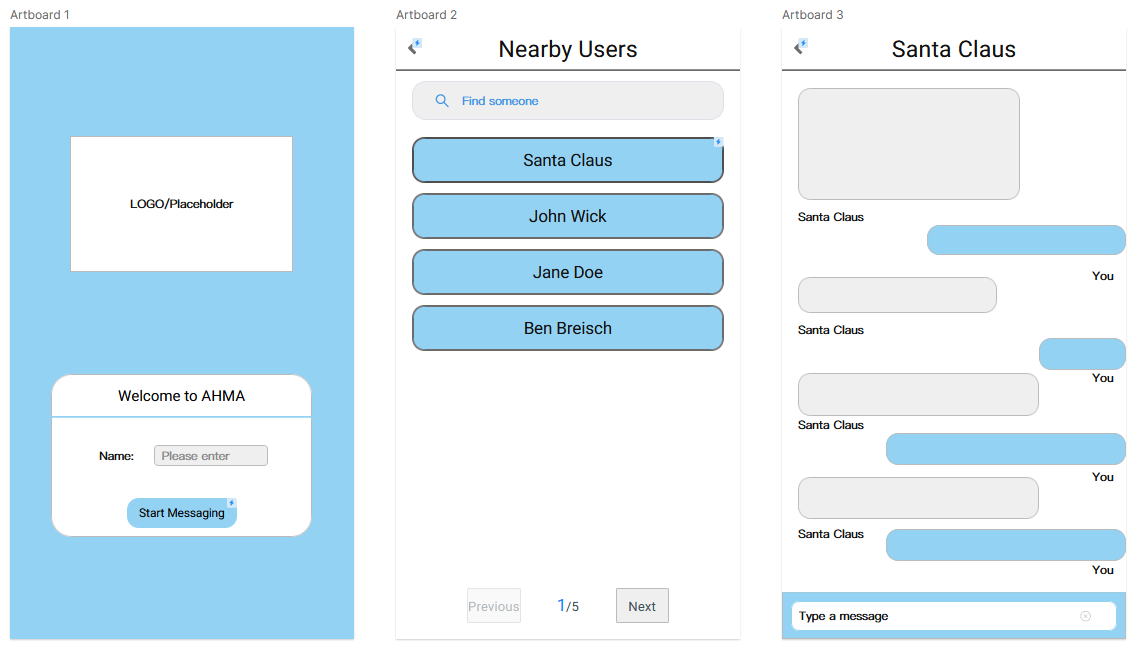
\includegraphics[scale=0.5]{wireframe.png} \\
\end{center}

Behind the scenes, this application uses a complex set of functions and internal storage structures. Devices  periodically broadcast beacon frames with routing information, tagged with usernames for each device. When the app is open on a device, it will listen for these beacon frames and update its list of nearby users accordingly. When a message is sent to a peer device, we use TCP for the best reliability. Conversations between users are stored on the device.

\section{Implementation}

As stated earlier in this report, the Ad-Hoc Messaging app was implemented in Kotlin using Android Studio. During development, we discovered that our app requires certain permissions to be given by the device owner. In order to ensure the proper permissions were granted, we added a fourth screen to the UI layout. This permission screen is shown to the user on startup if the app is lacking any permissions. This aids in development as a sanity check that any issues we run into are not permission-related.

\subsection{Front-End}
The front end was developed using Jetpack Compose, a built-in framework for Android Studio. Jetpack Compose is built around Composables, reusable units of code that compile into visual elements. The app uses about a dozen different composables, each written by us for UI elements such as buttons or text fields. Each screen in the app is a composable as well.
There are four separate screens on the app. 

\subsubsection{Permission Screen}

The permission screen is shown in Figure \ref{frontend:screens} at the end of this section. This screen is fairly simple. It shows a message that lets the user know that the app is missing the correct permissions. At the bottom of the page, there is a button that users can click on to be taken to the Android OS permission settings for the app. All users need to do is allow the correct permissions and go back to the app in order to be taken to the sign-in screen. This prevents users (and developers) from using the app without the proper permissions - which would cause errors and a bad user experience.

\subsubsection{Sign-In Screen}
The sign-in screen is shown in Figure \ref{frontend:screens} at the end of this section. Users are presented with the AI-generated logo for this app as well as a text-box to input their desired username. After entering a username, the user can click the sign-in button in order to kick off the back-end processes to start broadcasting frames and looking for other devices nearby.
\subsubsection{User Screen}

After a user clicks the sign-in button on the sign-in screen, many of the backend services are started. Once the back-end processes discover a nearby device running the app, the process adds the discovered device to the UI. The user can select the device in order to initiate a Wi-Fi Direct connection and transition to the chat screen.

\subsubsection{Chat Screen}
Opening the chat screen for a discovered device requires the Wi-Fi Direct connection to be open and error-free. Users are presented with the local chat history, pulled from the MongoDB database. Users can type and send new messages at any time while inside the chat screen. If a message is successfully sent, the contents will populate as a sent message in the UI. If the message does not successfully send, the user is notified and not added to the database.

\begin{figure}[h]
    \centering
    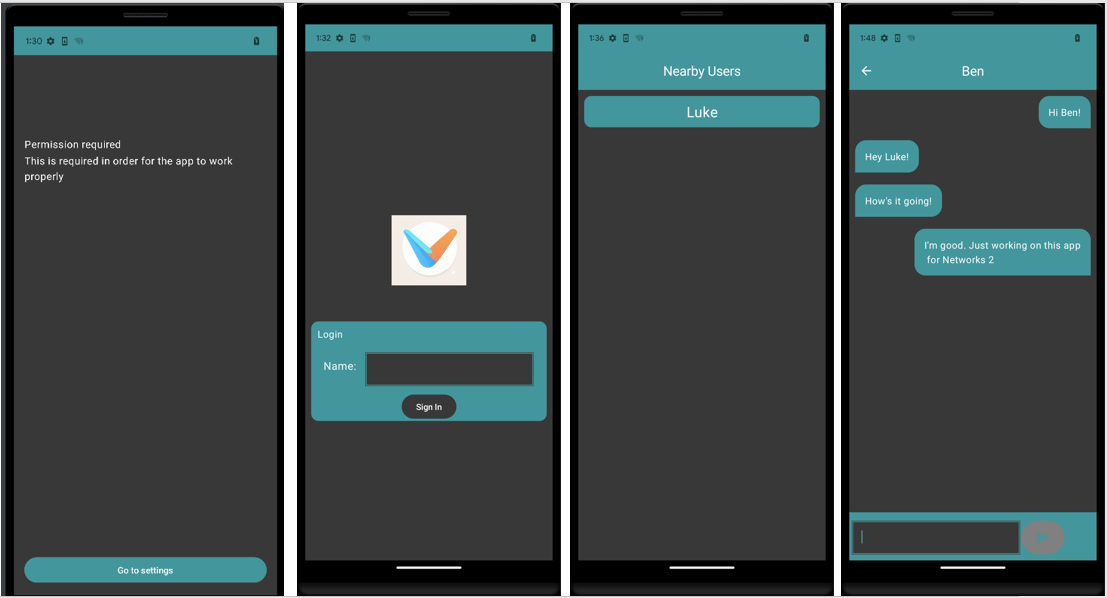
\includegraphics[width=6.5in]{screens.png}
    \caption{Permission, Sign-In, User, Chat Screens (Dark Mode)}
    \label{frontend:screens}
\end{figure}

\subsection{Back-End}
The back-end of this app is made up of many different services. These are required to run in separate threads by the Android API guidelines. The app is built around these services, requiring callbacks and asynchronous functions for much of the code. This increased the complexity of the code and lengthened development time.
\subsubsection{Service Advertisement}

After the user logs in, the app must broadcast that the device is ready for new connections. In order to do this, the Android Wi-Fi Direct API uses Domain Name Service - Service Discovery (DNS-SD). DNS-SD is an established protocol that allows for zero-configuration wide area service discovery. Other devices that have the app open listen for these DNS-SD broadcasts, and update their list of available devices accordingly. This requires a separate thread running on the device in order to check for updates in the background.

\subsubsection{Connection Protocol}
When a Wi-Fi Direct connection is initiated by a device, the other device is prompted with a system-level modal pop-up asking for permission to connect. When permission is allowed, both devices are connected in what Android's API calls a group. The initiating device is now the group owner, with a fixed IP address of 192.168.49.1. The other device is a group member, with a randomized last octet of the IP address, 192.168.49.1 - 192.168.49.255. This presents an issue for the group owner, who does not know the IP address of the other device. In order to fix that, when a device accepts an incoming Wi-Fi Direct connection, it will immediately send a HELLO message to the group owner, accompanied by the device's IP address. This HELLO message ensures both devices have each other's IP address. With addresses shared, devices are free to now send messages with each other over TCP, which is relatively trivial. Because we use TCP, we can ensure messages are delivered or the device is notified that the message was lost in transmission. Figure \ref{backend:proto} below shows the connection process.

\begin{figure}[h]
    \centering
    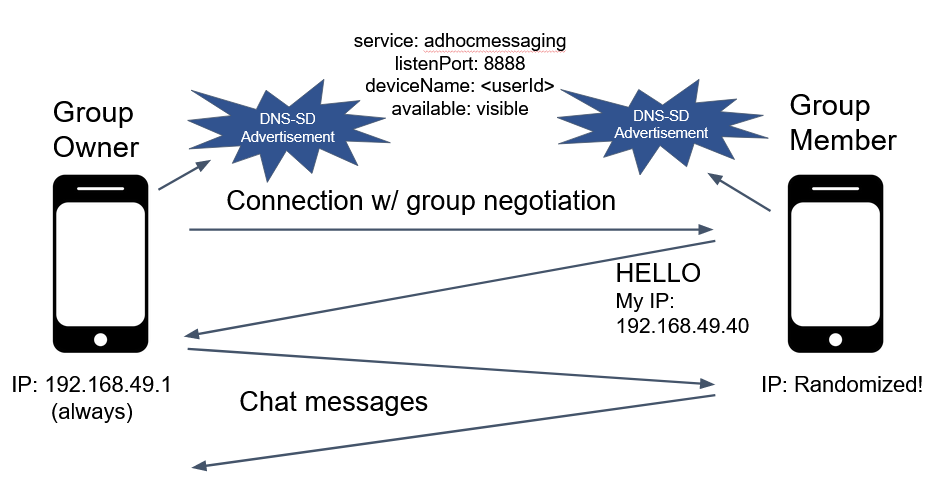
\includegraphics[width=5in]{proto.png}
    \caption{Connection Protocol w/ HELLO}
    \label{backend:proto}
\end{figure}

\subsubsection{Message Storage}

When messages are sent and received, they must be stored locally somewhere. In order to achieve this, the app uses a local SQLite database. Rather than actually implement our own SQLite database and objects in the program, we use Android's Room API which already implements SQLite. The app stores the content of the message, the timestamp of when it was sent/received, and the username of the user. It also stores whether the message was sent from the device, used for drawing the chat screen correctly. Table \ref{backend:sqlite} below shows the database schema used. 

\begin{table}[h]
    \begin{center}
    \begin{tabular}{|c|c|} \hline
        Field & Data type \\ \hline
        Chat ID & Integer \\
        Contact Name & String \\
        Source-Is-Me & Boolean \\
        Contents & String \\ \hline
    \end{tabular}
    \end{center}
    \caption{SQLite Database Schema}
    \label{backend:sqlite}
\end{table}


\subsection{Multi-Hop}

While our initial proposal set out requirements for multi-hop routing and creating a mesh network, we determined early on that this is not feasible. Because we are restricted to using Android's Wi-Fi Direct API, it would not make sense to do multi-hop routing using Wi-Fi Direct. We found that the association latency between clients is much too slow in order to accommodate any kind of mesh networking. For this reason, combined with the limited time horizon of the project, we decided not to pursue mesh networking using Wi-Fi Direct. We were also limited by access to only two Android phones that would have made testing a mesh Wi-Fi Direct network very challenging.

\section{Performance Evaluation}
%      \item What experiments are you going to run?
\subsection{Scenarios}

We performed all of our evaluation and experimentation on live android smart phones. One of our team members had a spare Wi-Fi Direct compatible Android phone and we acquired another such Android phone from Best Buy for testing. Since our application directly interacted with the hardware, we were unable to run it on anything but a genuine android phone. This therefore limited our testing to just the two android devices. To gain insight into our application's performance we tested it under the following scenarios:

\begin{itemize}
    \item Single-hop communication
    \item New user event
    \item Dropping user event
    \item High pace usage
    \item File/large messages
    \item Variable distance
\end{itemize}

The single-hop communication experiments were performed with the two android devices having a single connection between them. We also tested how quickly our application can adapt to topology changes such as users opening the app or closing the app. That in particular is especially important since people are rarely just using a single app continuously. Typical users will flip quickly between several different apps while using their phone or device. Additionally, we have tested the impact of high paced usage on network performance. Some users send messages back and forth as fast as their fingers can type and even do that with multiple different contacts. Most messaging apps also allow for users to send each other multimedia messages or files such as photos and videos so that capability has been tested as well. Finally, it is always important to study how the physical environment will impact performance. So we have run experiments at a variety of ranges from essentially 0 meters up to 10 meters. All of these scenarios have been combined into an array of experiments that we used to capture the performance of our app.

%   \item What criteria and metrics are you going to use to evaluate your solutions?
\subsection{Metrics}

For each experiment we have recorded the following metrics:

\begin{itemize}
    \item Throughput
    \item Latency
\end{itemize}

The throughput in this case is simply the data transmission rate between the two devices. So, all of the messages sent and received over a time time period measured in bits per second. The latency here depends on the situation, but in terms of messages it simply means the delay from when a message is sent on one device to when it is completely received on the other. We had originally hoped to decompose the latency into different components such as route acquisition, processing, potential queuing, transmission, propagation, re-transmission, and etc but all of those details are abstracted away in our implementation as the API handles it and functions as a black box.

\subsection{Criteria}

There are two key results we were looking for when performing these experiments. The first was to compare our app to other existing solutions. Specifically, we wanted to see if our approach of using WiFi-Direct performed better or worse than cellular messaging which is widely accepted and used. The second result is to discern if our solution meets the user's needs. Does it have the necessary throughput, latency, and reliability to provide a good experience for the casual user? That result tells us whether or not our solution is usable and functional.

The criteria for our first result is fairly straightforward. We simply compared our recorded metrics directly against cellular messaging on our phones. Generally speaking we found that cellular messaging has a latency of 1 second in ideal condition but could be much longer depending on location. On the other hand, the criteria for our second result was much less straightforward. There is no benchmark for the minimum performance required on a messaging app. So we evaluated the app against our own defined criteria of what is needed for a "good user experience".

Therefore our evaluation criteria are as follows:
\begin{itemize}
    \item Able to handle constant activity, fast paced messaging between users.
    \item Low latency
          \begin{itemize}
              \item Less than one second for text messages
              \item Less then ten seconds for files, pictures, or videos
          \end{itemize}
    \item Reliable delivery, data gets delivered unless destination is unreachable.
\end{itemize}

These are the basic requirements for any messaging app to be useful. If any one of these are missing then the user experience is miserable.
A messaging app needs to keep up with even the fastest typing user. We can put a character limit to restrict total message size, but that wouldn't stop a user from sending many large messages in quick succession. Therefore, it is important that the app can handle such usage. One speedy user shouldn't be able to cause network delay. We were able to manually test this ourselves by sending out messages as fast as possible and seeing if we observed an increase in network latency.

Since our app sends messages locally to a destination, rather than traveling through a complex network of infrastructure nodes, users will expect it to be very quick. Therefore, low latency is also a requirement. Specifically we hope to make it faster than even cellular under ideal conditions. Nobody likes to wait for something as simple as a message to send. Especially when some conversations are time sensitive. So the text messages themselves should send very quickly, with a small wait required for larger files.

Finally, messages need to be delivered. When a user sends a message they expect it to actually reach the destination. If that promise isn't upheld then that can cause confusion and frustration amongst users. If the destination is unreachable then the sending user needs to be alerted of this. This is a potential problem for our app as users could be hopping on and off the app at a rapid pace.

\subsection{Results}

To gather results we loaded our app onto the two Wi-Fi Direct capable android phones. We kept one of the phones hooked up to a laptop so we could collect its recorded logs for exact timing information. Then we proceeded to run each of the following experiments 10 times and average the outcomes. The first experiment shown in Figure \ref{results:message_latency} is the average latency of small and large messages during high pace usage of a single-hop connection between two phones. We decided to combine all of these scenarios to simulate what a real conversation between two users would be like in a worst case scenario. Both users would be sending both small text messages and also larger messages (we used up to 5 KB) while doing so at a high speed.

\begin{figure}[h!]
    \centering
    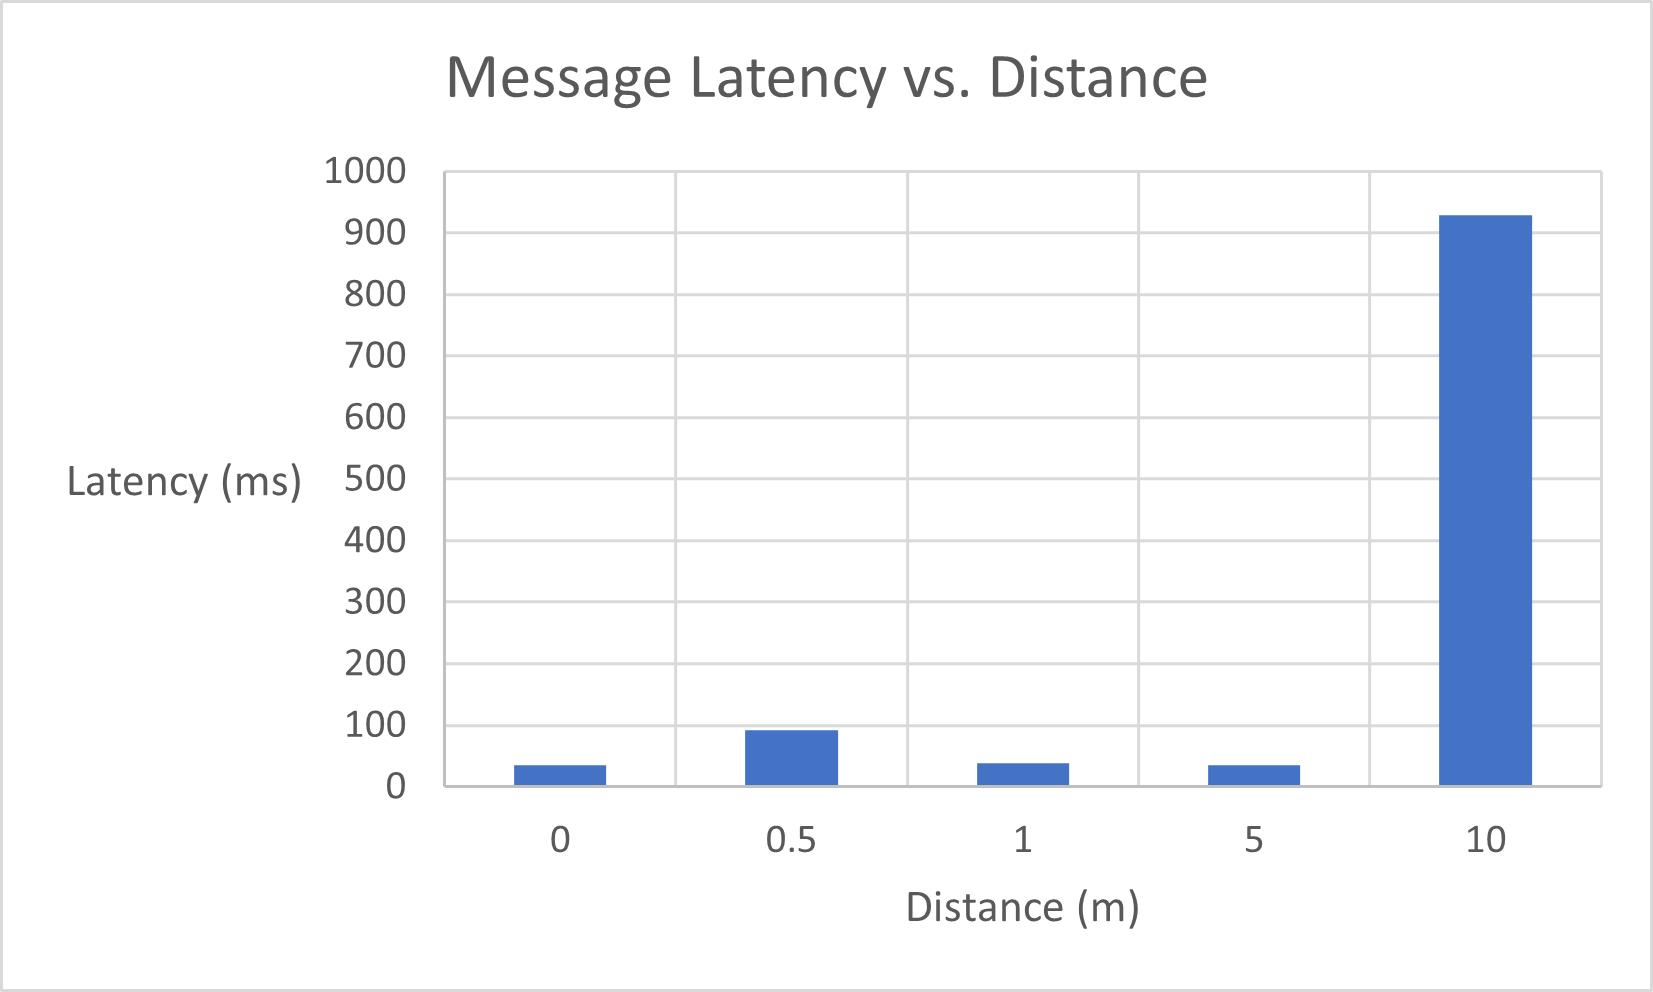
\includegraphics[width=4in]{message_latency_graph.png}
    \caption{Experiment 1: Message latency in milliseconds over varying distance in meters}
    \label{results:message_latency}
\end{figure}

Figure \ref{results:message_latency} shows the results of this experiment. There are two important results from this figure. The first is that distance significantly impacts latency. We can see that within 5 meters of distance the latency is below 100 ms or 0.1 seconds. This is extremely quick and basically instantaneous to the user. However, when we tested at a higher distance of 10 meters the latency immediately skyrocketed to a little over 900 ms or 0.9 seconds. This really emphasizes that Wi-Fi Direct is meant for local communication. The second result is that despite being sensitive to distance, this application is still extremely quick. Even our worst latency measurement is still below a second. Which means that our application successfully meets our criteria for fast-paced usage and also latency of less than one second for text messages.

\begin{figure}[h!]
    \centering
    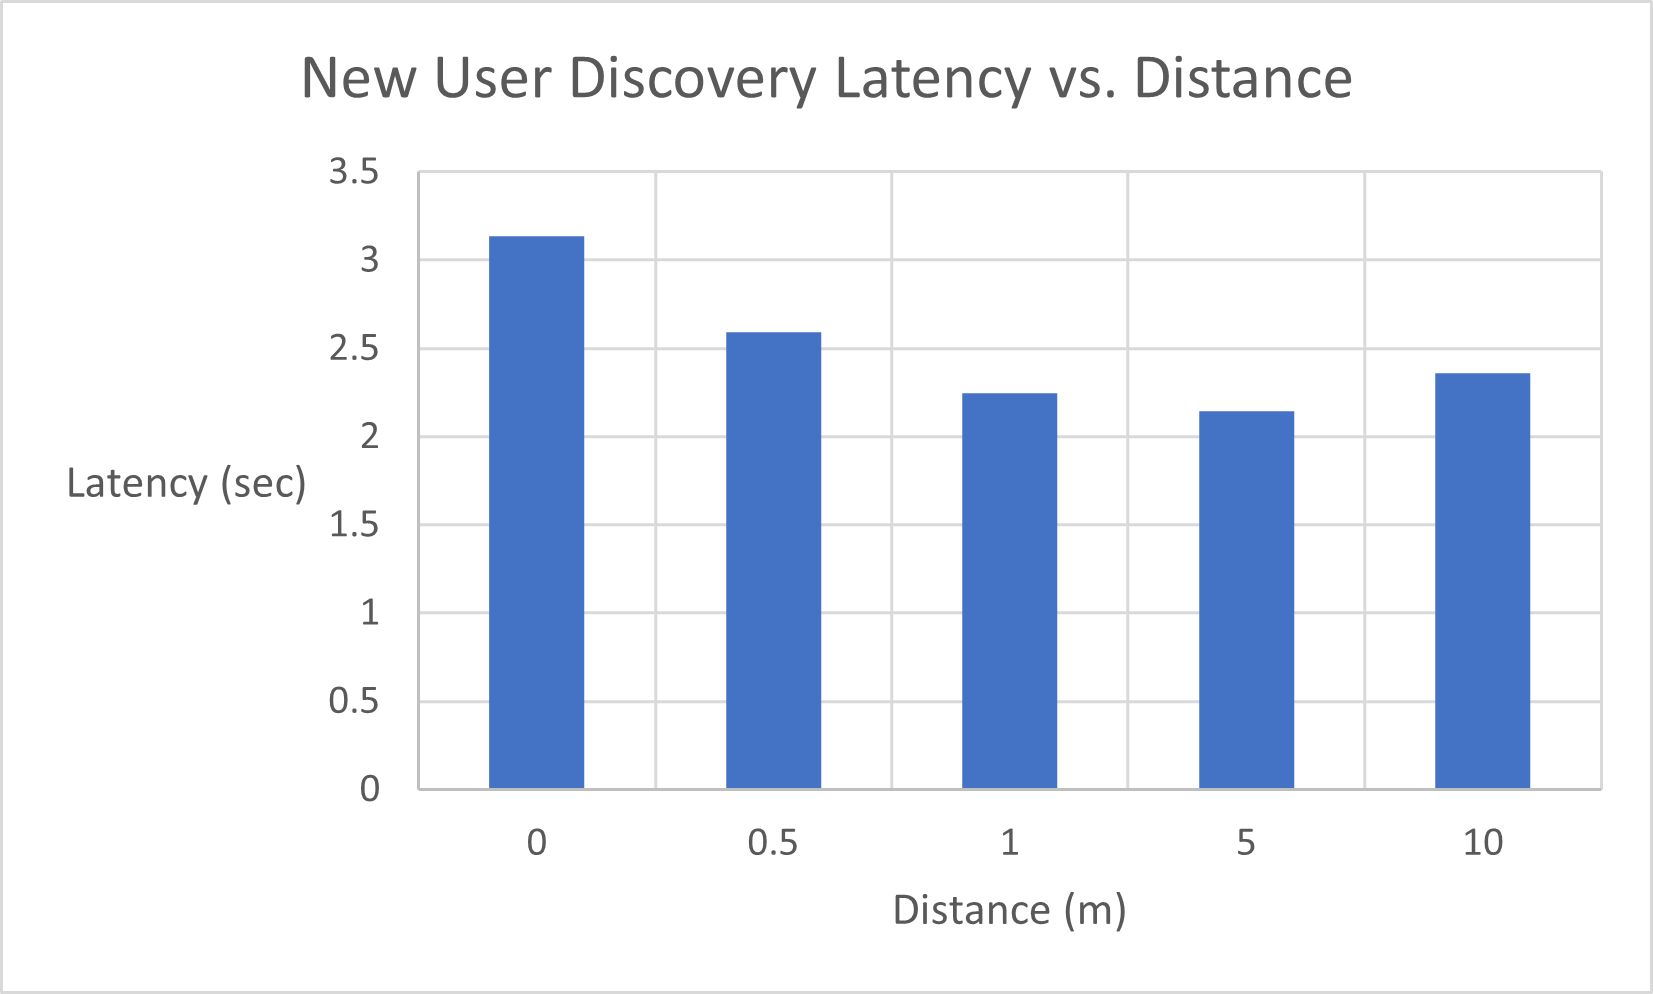
\includegraphics[width=4in]{new_user_dicovery_graph.png}
    \caption{Experiment 2: New user discovery latency in seconds over varying distance in meters}
    \label{results:new_user}
\end{figure}

Figure \ref{results:new_user} shows the latency from when a new device login occurs to when the other devices discover the new device. In the context of our application this represents the delay that a user has to endure after opening the app until other users notice that they are available to message with. This was tested by having one android device completely logged in and listening for peer devices running the app then starting the app on the other phone and recording the delay till the first phone notices the second one. As seen in the figure this metric has an interesting relationship with distance. The fastest new user discovery occurs when the devices are separated by 5 meters and it increases with any change with distance from that point. As mentioned in our implementation section the user discovery relies on service advertisements being sent out from each device running the app. When the devices are too close there seems to be some interference or something similar which delays user discovery.

\begin{figure}[h!]
    \centering
    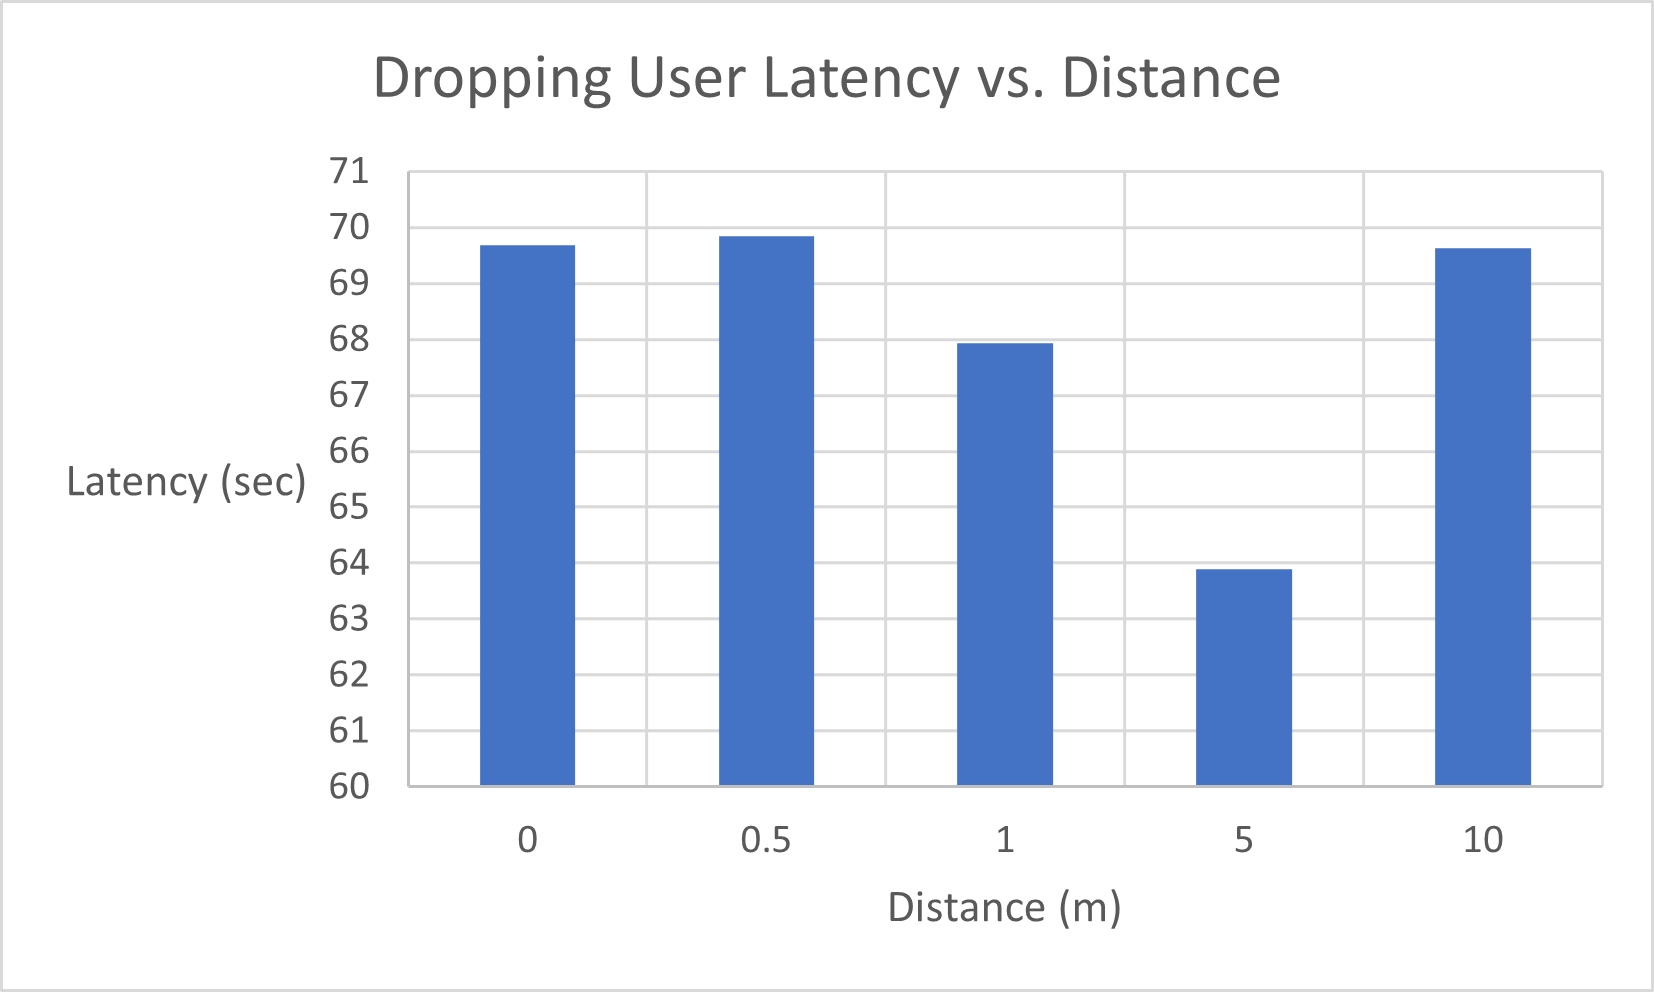
\includegraphics[width=4in]{dropping_user_latency_graph.png}
    \caption{Experiment 3: Dropping user latency in seconds over varying distance in meters}
    \label{results:dropping_user}
\end{figure}

Figure \ref{results:dropping_user} shows the latency between when a user closes the app and when other devices notice that device is no longer available for connection. This is represented in our app by having that user disappear from other device's "Nearby Users" screen. There is no strong relationship between distance and this metric as it varies without any real pattern. The main takeaway from this is that the delay here is extremely high. It takes around 69 seconds for other devices to alert our application that a nearby user has dropped out of range or stopped using the app. This may be because the protocol is very tolerant to intermittent disconnections and wireless transmission issues, so it allows a certain grace period of not hearing any service advertisement messages before it determines that the peer device is gone. In the case where a user is trying to use multiple apps at once this delay could actually be helpful. However it is important to note that if two devices are directly connected in a Wi-Fi Direct group and one leaves the group then the other device is immediately alerted that they've lost connection.

\begin{figure}[h!]
    \centering
    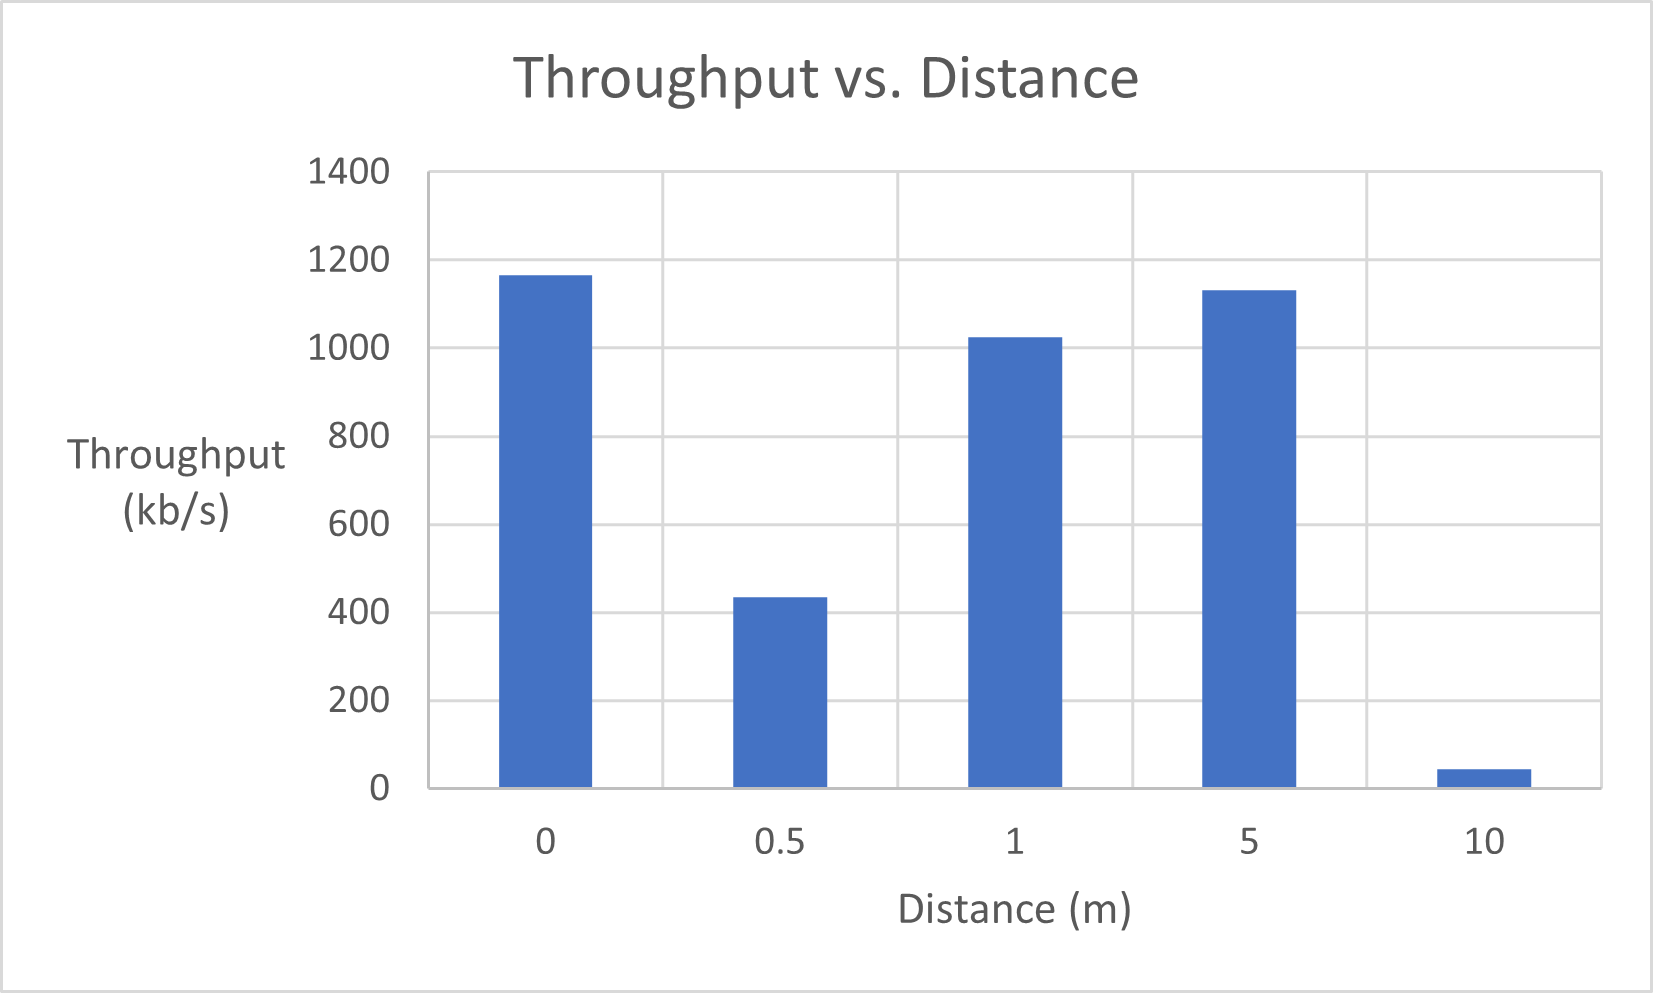
\includegraphics[width=4in]{throughput_graph.png}
    \caption{Experiment 4: Network throughput in kbps over varying distance in meters}
    \label{results:throughput}
\end{figure}

Figure \ref{results:throughput} shows the relationship between network throughput and distance for a single-hop connection between two android devices. This was tested by sending several moderately large text files between the two devices and measuring the latency in delivery much like in figure \ref{results:message_latency}. Then based off the file length and latency we were able to calculate a rough measurement of network throughput over varying distances. We observed a peak average throughput of almost 1.2 Mbps when the devices were right next to each other at 0 meters. The rest of the measurements roughly reflect the latency values observed in figure \ref{results:message_latency}. Where distances of 1 and 5 meters were similar to 0 meters and throughput severely drops when we tested at 10 meters distance. At that distance we observed around 43 kbps. Which is still fast enough to send any text message or small file, but would struggle with larger files. 

The important question here is does this throughput meet our soft criteria for sending files, pictures, or videos? Well if we look at the peak case of 1.165 Mbps throughput then our app could successfully send files, picures, and videos of up to 11.65 Mb or 1.456 MB within 10 seconds. Considering that a high-resolution photograph is at least 2MB then this criteria is not being fully met. It could handle smaller files and lower-resolution photographs, but it would take more than 10 seconds to send a higher-resolution photograph or videos.

During our experimentation we also found two further results. One is that we never experienced messages not being delivered after a connection was established. This is because our application uses TCP for communication which we know guarantees reliable delivery with re-transmission. Therefore our last criteria point was being met without any further work from us. The second result is that our app worked up to at least a distance of 50 meters. We were able to get consistent and relatively quick messages sent both ways but were unable to test it further. We assume this means our app possesses a similar range to traditional Wi-Fi as it uses the same hardware.

\section{Conclusion}

% Did our app meet the criteria and requirements we set forth?

When someone sends a message through SMS or Apple's iMessage, the sent data travels from the originating phone to its corresponding cell tower and then through a complex series of intermediate infrastructure nodes before reaching its destination. In general this is appreciated because it supports long-distance messaging to anyone in the world. However, not every message needs to take such a convoluted path. If both the source and destination devices are in the same location within meters of each other then the typical delivery path just increases latency and creates unnecessary network overhead. Especially if both devices are in a location with poor cell service. In this report we investigated one possible solution to this problem by developing a peer-to-peer messaging app for Android that uses Wi-Fi Direct for local communication. The app was developed using Android’s Studio Software Development Kit in Kotlin. We successfully implemented our app on two android phones and were able to test the performance according to several criteria. We discovered the following important results:

\begin{table}
    \centering
    \begin{tabular}{|c|c|}
        \hline
        Requirement & Met?\\
        \hline \hline
        Able to handle constant, fast paced activity & Yes\\
        \hline
        Less than one second latency for text messages & Yes\\
        \hline
        Less than ten seconds for files, pictures, or videos & Partially\\
        \hline
        Reliable delivery & Yes\\
        \hline
    \end{tabular}
    \caption{Criteria satisfaction}
    \label{tab:conclusions}
\end{table}

As seen in Table \ref{tab:conclusions}, our application met almost all of our criteria for what constitutes a good messaging app. It also shows that our application is at least comparable to existing cellular messaging when at close range. The only requirement it didn't meet was the latency on larger files. We found that our application could only handle files up to 1.456 MB within 10 seconds. Which isn't enough for some high-resolution photos or videos, but it can still handle smaller files fairly quickly. So overall we found that a messaging application using Wi-Fi Direct performs well for single-hop communication with it currently being unable to support multi-hop communication.

\renewcommand{\refname} {\section{References}}
\bibliographystyle{acm}
\bibliography{refs}{}

\end{document}
